%%%%%%%%%%%%%%%%%%%%%%%%%%%%%%%%%%%%%%%%%%%%%%%%%%%%%%%%%%%%%%%%%%%%%%%%%%% 
% 
% Generic template for the anteproyectos of TFC/TFM/TFGs
% 
% $Id: anteproyecto.tex,v 1.6 2018/09/11 12:23:48 macias Exp $
% 
% By:
%  + Javier Macías-Guarasa. 
%    Departamento de Electrónica
%    Universidad de Alcalá
%  + Roberto Barra-Chicote. 
%    Departamento de Ingeniería Electrónica
%    Universidad Politécnica de Madrid   
% 
% Based on original sources by Roberto Barra, Manuel Ocaña, Jesús Nuevo,
% Pedro Revenga, Fernando Herránz and Noelia Hernández. Thanks a lot to
% all of them, and to the many anonymous contributors found (thanks to
% google) that provided help in setting all this up.
% 
% See also the additionalContributors.txt file to check the name of
% additional contributors to this work.
% 
% If you think you can add pieces of relevant/useful examples,
% improvements, please contact us at (macias@depeca.uah.es)
% 
% You can freely use this template and please contribute with
% comments or suggestions!!!
% 
%%%%%%%%%%%%%%%%%%%%%%%%%%%%%%%%%%%%%%%%%%%%%%%%%%%%%%%%%%%%%%%%%%%%%%%%%%% 

% This is for rubber to clean additional files
% rubber: clean anteproyecto.acn anteproyecto.acr anteproyecto.alg anteproyecto.cod anteproyecto.ist anteproyecto.out anteproyecto.sbl anteproyecto.slg anteproyecto.sym anteproyecto.lor

\documentclass[11pt,a4paper,oneside]{article}

%%%%%%%%%%%%%%%%%%%%%%%%%%%%%%%%%%%%%%%%%%%%%%%%%%%%%%%%%%%%%%%%%%%%%%%%%%% 
% BEGIN Preamble and configuration section
% 

\usepackage{tikz}
\usetikzlibrary{positioning}

\input{../Config/preamble.tex}    % DO NOT TOUCH THIS LINE. You can edit
                                  % the file to modify some default settings

\input{../Config/myconfig.tex}    % DO NOT TOUCH THIS LINE, but EDIT THIS FILE
                                  % to set your specific settings (related
                                  % to the document language, your degree,
                                  % document details (such as title, author
                                  % (you), your email, name of the tribunal
                                  % members, document year, keyword and
                                  % palabras clave) and link colors), and
                                  % define your commonly used commands
                                  % (some examples are provided).

\input{../Config/postamble.tex}   % DO NOT TOUCH THIS LINE. Yes, I know,
                                  % "postamble" is not a valid word... :-)
%
% END Preamble and configuration section
%%%%%%%%%%%%%%%%%%%%%%%%%%%%%%%%%%%%%%%%%%%%%%%%%%%%%%%%%%%%%%%%%%%%%%%%%%%

% path to directories containing images
\graphicspath{{../Book/logos/}{../Book/figures/}{../Book/diagrams/}} % Edit this to your
                                  % needs. Only logos is really required
                                  % when you generate your own content.
% 
% END Preamble and configuration section
%%%%%%%%%%%%%%%%%%%%%%%%%%%%%%%%%%%%%%%%%%%%%%%%%%%%%%%%%%%%%%%%%%%%%%%%%%% 

\title{Anteproyecto de \myWorkTypeFull}        % DO NOT TOUCH THIS LINE
\date{\myThesisProposalDate}                         % DO NOT TOUCH THIS LINE
\author{\myAuthorFullName}

%%%%%%%%%%%%%%%%%%%%%%%%%%%%%%%%%%%%%%%%%%%%%%%%%%%%%%%%%%%%%%%%%%%%%%%%%%% 
% Let's start with the real stuff
%%%%%%%%%%%%%%%%%%%%%%%%%%%%%%%%%%%%%%%%%%%%%%%%%%%%%%%%%%%%%%%%%%%%%%%%%%% 
\begin{document}                                   % DO NOT TOUCH THIS LINE

%%%%%%%%%%%%%%%%%%%%%%%%%%%%%%%%%%%%%%%%%%%%%%%%%%%%%%%%%%%%%%%%%%%%%%%%%%% 
% BEGIN within-document configuration, frontpage and cover pages generation
% 

% Set Language dependent issues that must be set after \begin{document}
\input{../Config/setlanguagedependentissues.tex} % DO NOT TOUCH THIS LINE
                                                 % NOR THE FILE

% 
% END within-document configuration, frontpage and cover pages generation
%%%%%%%%%%%%%%%%%%%%%%%%%%%%%%%%%%%%%%%%%%%%%%%%%%%%%%%%%%%%%%%%%%%%%%%%%%% 

\maketitle

\begin{description}                               % DO NOT TOUCH THIS LINE
\item[\expandafter\makefirstuc\expandafter{\wordAutorOrAutora}:] \myAuthorFullName                       % DO NOT TOUCH THIS LINE
\item[\expandafter\makefirstuc\expandafter{\wordTutorOrTutores}:] \myAdvisors                   % DO NOT TOUCH THIS LINE
  \item[Titulación:] \myDegreefull                % DO NOT TOUCH THIS LINE
  \item[Título:] \myBookTitleSpanish              % DO NOT TOUCH THIS LINE
  \ifthenelse{\equal{\myLanguage}{english}}       % DO NOT TOUCH THIS LINE
  {                                               % DO NOT TOUCH THIS LINE
  \item[Título en inglés:] \myBookTitleEnglish    % DO NOT TOUCH THIS LINE
  }                                               % DO NOT TOUCH THIS LINE
  {                                               % DO NOT TOUCH THIS LINE
  }                                               % DO NOT TOUCH THIS LINE
\item[Departamento:] \myDepartment                % DO NOT TOUCH THIS LINE
\end{description}                                 % DO NOT TOUCH THIS LINE

%\tableofcontents

%%%%%%%%%%%%%%%%%%%%%%%%%%%%%%%%%%%%%%%%%%%%%%%%%%%%%%%%%%%%%%%%%%%%%%%%%%% 
%%%%%%%%%%%%%%%%%%%%%%%%%%%%%%%%%%%%%%%%%%%%%%%%%%%%%%%%%%%%%%%%%%%%%%%%%%% 
%%%%%%%%%%%%%%%%%%%%%%%%%%%%%%%%%%%%%%%%%%%%%%%%%%%%%%%%%%%%%%%%%%%%%%%%%%% 
%%%%%%%%%%%%%%%%%%%%%%%%%%%%%%%%%%%%%%%%%%%%%%%%%%%%%%%%%%%%%%%%%%%%%%%%%%% 
%%%%%%%%%%%%%%%%%%%%%%%%%%%%%%%%%%%%%%%%%%%%%%%%%%%%%%%%%%%%%%%%%%%%%%%%%%% 
%%%%%%%%%%%%%%%%%%%%%%%%%%%%%%%%%%%%%%%%%%%%%%%%%%%%%%%%%%%%%%%%%%%%%%%%%%% 
%%%%%%%%%%%%%%%%%%%%%%%%%%%%%%%%%%%%%%%%%%%%%%%%%%%%%%%%%%%%%%%%%%%%%%%%%%% 
% BEGIN Normal sections. Edit/modify all within this section

\section{Introducción}
\label{sec:introduccion}

La salud mental se ha convertido en uno de los principales desafíos del siglo XXI, con más de mil millones de personas afectadas por algún trastorno mental según estimaciones recientes de la Organización Mundial de la Salud \cite{BillionPeopleLiving}. Entre los trastornos más prevalentes se encuentran la ansiedad, la depresión y los trastornos alimentarios, los cuales generan un profundo impacto personal, social y económico. Paralelamente, el uso masivo de redes sociales, plataformas digitales y servicios de mensajería ha generado nuevas oportunidades para analizar el lenguaje escrito como indicador del estado psicológico de las personas. En este contexto, los avances en procesamiento del lenguaje natural (PLN) e inteligencia artificial han abierto la puerta a sistemas capaces de detectar señales tempranas de malestar emocional a partir de textos.

Durante la última década, los modelos basados en \textit{transformers} han impulsado un cambio significativo en el PLN, permitiendo avances notables en tareas como la clasificación de texto, el análisis semántico y la comprensión contextual profunda \cite{vaswaniAttentionAllYou2017}. Modelos como BERT \cite{devlinBERTPretrainingDeep2019} han demostrado gran eficacia en tareas supervisadas del ámbito de la salud mental, mientras que los actuales Grandes Modelos de Lenguaje (LLM), como GPT-5, ofrecen capacidades avanzadas de razonamiento y análisis contextual que permiten explorar nuevas aproximaciones metodológicas.

Los trabajos más recientes en este campo han comenzado a explorar el uso de Grandes Modelos de Lenguaje para la detección automática de indicadores psicológicos. Por un lado, Danner et al.\ investigan métodos basados en GPT para mejorar la identificación de depresión a partir de texto, mostrando que los LLM pueden superar a modelos tradicionales \cite{dannerAdvancingMentalHealth2023}. Por otro lado, Liu et al.\ presentan un enfoque que utiliza LLMs optimizados para el cribado de depresión y ansiedad, demostrando mejoras significativas en sensibilidad y capacidad de interpretación \cite{liuEnhancedLargeLanguage2025}. A pesar de estos avances, la mayoría de estudios continúan centrados casi exclusivamente en la depresión, mientras que los trabajos dedicados a la ansiedad u otros trastornos---como los alimentarios---siguen siendo escasos. Además, la gran mayoría emplea datos en inglés, lo que dificulta su aplicación en contextos hispanohablantes.

El presente trabajo propone un análisis comparativo entre un modelo más tradicional basado en BERT y diversos modelos de última generación (LLMs) para la detección automática de ansiedad, depresión y trastornos alimentarios en textos escritos en español. Este proyecto se distingue de trabajos anteriores al emplear datasets específicos en español, integrar modelos contemporáneos como GPT-5 y abordar simultáneamente tres categorías clínicas en lugar de centrarse únicamente en la depresión, ampliando así el alcance y la relevancia de la investigación. Asimismo, este trabajo se orienta exclusivamente a tareas de cribado y apoyo al análisis temprano, sin pretender en ningún caso sustituir el juicio clínico ni el diagnóstico de un profesional de la salud mental.


\section{Objetivos}
\label{sec:objetivos-y-campo}

El objetivo general de este TFG es evaluar la capacidad de distintos modelos de procesamiento del lenguaje natural (PLN) para detectar de forma automática indicadores de ansiedad, depresión y trastornos alimentarios en textos escritos en español.

A partir de este objetivo principal, se plantean los siguientes objetivos específicos:

\begin{itemize}
	\item Analizar y preprocesar un dataset en español que contenga textos anotados con presencia o ausencia de ansiedad, depresión y trastornos alimentarios.
	\item Entrenar y evaluar un modelo basado en BERT, aplicando técnicas de \textit{fine-tuning} para tareas de clasificación.
	\item Aplicar LLMs mediante \textit{zero-shot prompting}, utilizando las APIs de distintos proveedores de modelos avanzados, con el fin de predecir la presencia de los distintos trastornos sin necesidad de reentrenamiento.
	\item Comparar de forma sistemática los resultados obtenidos por ambos enfoques, analizando métricas como precisión, \textit{recall}, F1-score y capacidad de generalización.
	\item Reflexionar sobre las ventajas, limitaciones y posibles sesgos derivados del uso de modelos de lenguaje en tareas relacionadas con la salud mental.
\end{itemize}

\subsection{Campo de aplicación}

El trabajo se sitúa en el ámbito del cribado automático de señales tempranas de posibles trastornos de salud mental. Los modelos evaluados tienen un propósito exclusivamente orientado a la detección inicial y al apoyo a la investigación, sin sustituir la valoración de un profesional. Su aplicación potencial incluye sistemas de monitorización en plataformas digitales o redes sociales, herramientas de apoyo para estudios en psicología computacional y aplicaciones de prevención donde sea útil identificar posibles indicadores de malestar emocional de forma preliminar.

\section{Descripción del trabajo}
\label{sec:descr-del-trab}

El trabajo analizará la capacidad de distintos modelos de procesamiento del lenguaje natural (PLN) para detectar posibles indicios de ansiedad, depresión y trastornos alimentarios en textos en español utilizando el \textit{dataset} MentalRiskES \cite{marmolromeroMentalRiskESNewCorpus2024}. Para ello se compararán dos enfoques: un modelo basado en BERT entrenado mediante \textit{fine-tuning} y varios Grandes Modelos de Lenguaje (LLMs) accesibles mediante API. El estudio incluirá tanto clasificación binaria (presencia o ausencia de cada trastorno) como clasificación multiclase, con el fin de evaluar posibles confusiones entre categorías y valorar la utilidad de estos sistemas como herramientas de cribado.

\subsection{Fases del trabajo}

\begin{enumerate}
	\item \textbf{Análisis y preparación del \textit{dataset} MentalRiskES}.  
	Se revisará la estructura del \textit{dataset}, dividido en tres subconjuntos correspondientes a ansiedad, depresión y trastornos alimentarios, analizando la distribución de clases y el formato de los textos. Posteriormente, se realizará el preprocesamiento necesario (limpieza y normalización) y la preparación de los conjuntos de validación y prueba para los dos escenarios de clasificación: binaria y multiclase.
	
	\item \textbf{Entrenamiento del modelo BERT}.  
	Se seleccionará una variante adecuada para español y se aplicará \textit{fine-tuning} para:
	\begin{itemize}
		\item Clasificación binaria: un modelo para ansiedad, otro para depresión y otro para trastornos alimentarios.
		\item Clasificación multiclase: un único modelo capaz de distinguir entre los tres trastornos o la ausencia de ellos.
	\end{itemize}
	El rendimiento se evaluará mediante precisión, \textit{recall} y F1-score.
	
	\item \textbf{Investigación y selección de LLMs}.  
	Se llevará a cabo una fase de exploración para seleccionar modelos concretos dentro de los siguientes proveedores: OpenAI, Google Gemini, Claude (Anthropic), DeepSeek y Mistral, analizando sus capacidades y limitaciones.
	
	\item \textbf{Evaluación de LLMs mediante \textit{zero-shot prompting}}.  
	Se diseñarán \textit{prompts} específicos para que cada LLM realice:
	\begin{itemize}
		\item Clasificación binaria: predicción independiente de ansiedad, depresión y trastornos alimentarios.
		\item Clasificación multiclase: identificación del trastorno predominante o ausencia de trastornos.
	\end{itemize}
	Las predicciones se evaluarán con las mismas métricas que el modelo BERT.
	
	\item \textbf{Comparación y análisis final}.  
	Se compararán ambos enfoques estudiando métricas globales, patrones de error, confusiones entre trastornos y diferencias entre modelos entrenados y LLMs en \textit{zero-shot}.
\end{enumerate}

\setcounter{figure}{0}
\begin{figure}[tphb]
  \centering
  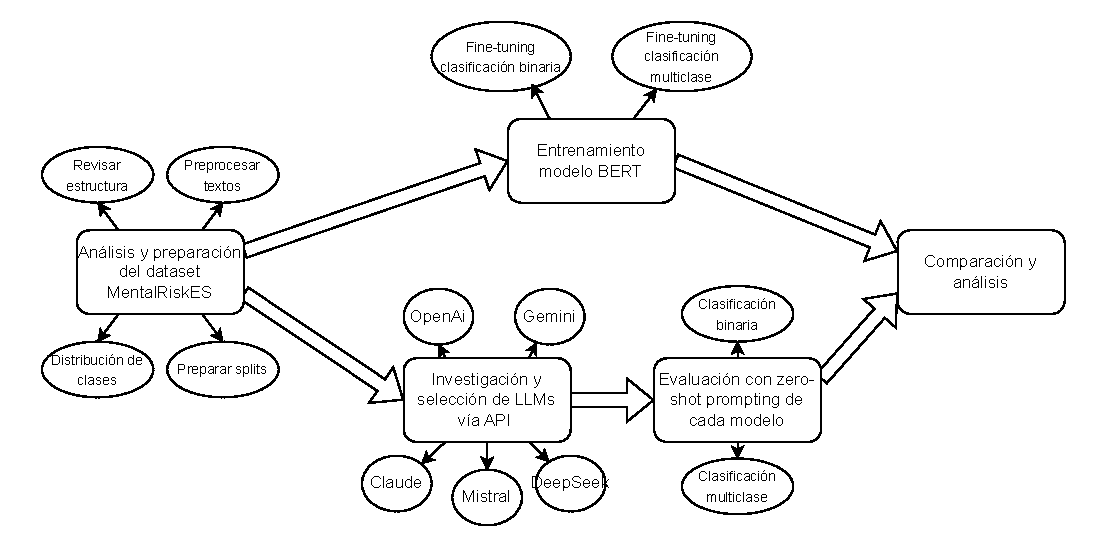
\includegraphics[width=6in]{DesarrolloTFG.pdf}
  \label{fig:arquitectura}
  \caption{Diagrama general del flujo de trabajo.}
\end{figure}


\section{Metodología y plan de trabajo}
\label{sec:metodologia-y-plan}

La metodología del trabajo se basa en un enfoque experimental dividido en varias etapas consecutivas y parcialmente solapadas. Cada fase corresponde a un hito concreto del TFG y sigue un flujo lógico desde el análisis del dataset hasta la evaluación final de los modelos.

\subsection{Etapas del trabajo}

\begin{enumerate}
	\item \textbf{Revisión inicial y planificación} (3 semanas).  
	Revisión bibliográfica, concreción del enfoque metodológico (clasificación binaria y multiclase) y organización del calendario de trabajo.
	
	\item \textbf{Análisis y preparación del \textit{dataset} MentalRiskES} (3 semanas).  
	Estudio de la estructura del \textit{dataset} y sus tres subconjuntos (ansiedad, depresión y trastornos alimentarios). Preprocesamiento de los textos (limpieza y normalización) y preparación de los conjuntos de validación y prueba.
	
	\item \textbf{Entrenamiento del modelo BERT con \textit{fine-tuning}} (6 semanas).  
	Selección de una variante adecuada para español (como BETO). Entrenamiento del modelo tanto para clasificación binaria (tres modelos independientes) como para clasificación multiclase (un único modelo). Evaluación mediante métricas estándar como precisión, \textit{recall} y F1-score.
	
	\item \textbf{Investigación y selección de LLMs} (2 semanas).  
	Exploración de modelos disponibles mediante API en distintos proveedores: OpenAI, Google Gemini, Claude (Anthropic), DeepSeek y Mistral. Selección de modelos y diseño inicial de los \textit{prompts} necesarios para la evaluación.
	
	\item \textbf{Evaluación de LLMs mediante \textit{zero-shot prompting}} (8 semanas).  
	Obtención de predicciones tanto para clasificación binaria como para clasificación multiclase, utilizando los mismos conjuntos de prueba empleados en el modelo BERT. Cálculo de métricas de rendimiento para cada modelo.
	
	\item \textbf{Comparación global y análisis crítico} (3 semanas).  
	Comparación cuantitativa entre los dos enfoques, análisis de errores y confusiones entre trastornos, así como reflexión sobre implicaciones éticas y limitaciones del uso de modelos de lenguaje en tareas de cribado de salud mental.
	
	\item \textbf{Redacción de la memoria y conclusiones} (4 semanas).  
	En este punto, ya se habrán ido documentando las etapas anteriores en la memoria. Queda elaborar los capítulos finales del documento, discusión de resultados y propuestas de mejora y líneas de trabajo futuras.
\end{enumerate}

\begin{figure}[H]
	\centering
	
	\begin{ganttchart}[
		title height=1,
		x unit=0.05cm,
		y unit title=0.6cm,
		y unit chart=0.5cm,
		bar height=0.5,
		vgrid={*{6}{draw=none}, *1{draw, dotted}},
		hgrid,
		time slot format=isodate,
		group label font=\bfseries\footnotesize,
		bar label font=\footnotesize,
		title label font=\footnotesize,
		group/.append style={fill=gray!75},
		group peaks height=0.3, % Increase the height of the vertical marks
		group peaks width=2, % Increase the width of the vertical marks
		group peaks tip position=0 % Center the vertical marks
		]{2025-10-27}{2026-05-17}
		
		% Calendar
		\gantttitlecalendar{year, month} \\
		
		% ---------------------------
		% 1. REVISION INICIAL
		% ---------------------------
		\ganttgroup{Revisión inicial y planificación}{2025-10-27}{2025-11-17} \\
		
		\ganttbar{Revisión bibliográfica}{2025-10-27}{2025-11-02} \\
		\ganttbar{Definición detallada del enfoque}{2025-11-03}{2025-11-09} \\
		\ganttbar{Redacción del anteproyecto}{2025-11-10}{2025-11-17} \\
		
		% ---------------------------
		% 2. ANALISIS Y PREPARACION
		% ---------------------------
		\ganttgroup{Análisis y preparación del dataset}{2025-11-18}{2025-12-07} \\
		
		\ganttbar{Estudio de la estructura del dataset}{2025-11-17}{2025-11-27} \\
		\ganttbar{Limpieza y normalización de textos}{2025-11-27}{2025-12-04} \\
		\ganttbar{Preparación de validación y prueba}{2025-12-04}{2025-12-07} \\
		
		% ---------------------------
		% 3. ENTRENAMIENTO BERT
		% ---------------------------
		\ganttgroup{Entrenamiento modelo BERT}{2025-12-08}{2026-01-18} \\
		
		\ganttbar{Selección de variante BERT}{2025-12-08}{2025-12-10} \\
		\ganttbar{Entr. binaria (ansiedad)}{2025-12-11}{2025-12-19} \\
		\ganttbar{Entr. binaria (depresión)}{2025-12-19}{2025-12-27} \\
		\ganttbar{Entr. binaria (TCA)}{2025-12-27}{2026-01-04} \\
		\ganttbar{Entrenamiento multiclase}{2026-01-02}{2026-01-15} \\
		\ganttbar{Evaluación BERT}{2026-01-15}{2026-01-18} \\
		
		% ---------------------------
		% 4. INVESTIGACIÓN LLMs
		% ---------------------------
		\ganttgroup{Investigación y selección de LLMs}{2026-01-19}{2026-02-01} \\
		
		\ganttbar{Exploración de modelos}{2026-01-19}{2026-01-24} \\
		\ganttbar{Análisis de capacidades y costes}{2026-01-24}{2026-01-28} \\
		\ganttbar{Diseño preliminar de prompts}{2026-01-28}{2026-02-01} \\
		
		% ---------------------------
		% 5. ZERO-SHOT LLMs
		% ---------------------------
		\ganttgroup{Evaluación con LLMs (zero-shot)}{2026-02-02}{2026-03-29} \\
		
		\ganttbar{Predicciones binarias}{2026-02-02}{2026-03-08} \\
		\ganttbar{Predicciones multiclase}{2026-03-08}{2026-03-22} \\
		\ganttbar{Obtención de métricas}{2026-03-22}{2026-03-29} \\
		
		% ---------------------------
		% 6. COMPARACION
		% ---------------------------
		\ganttgroup{Comparación y análisis crítico}{2026-03-29}{2026-04-19} \\
		
		\ganttbar{Comparación cuantitativa}{2026-03-29}{2026-04-10} \\
		\ganttbar{Análisis de errores y confusiones}{2026-04-10}{2026-04-17} \\
		\ganttbar{Revisión ética y limitaciones}{2026-04-17}{2026-04-19} \\
		
		% ---------------------------
		% 7. REDACCION FINAL
		% ---------------------------
		\ganttgroup{Redacción memoria y conclusiones}{2025-11-18}{2026-05-17} \\
		
		\ganttbar{Documentación}{2025-11-18}{2026-05-17} \\
		\ganttbar{Conclusiones y revisión}{2026-04-20}{2026-05-17} \\
		
	\end{ganttchart}
	
	\caption{Diagrama de Gantt de la planificación del trabajo.}
	\label{fig:gantt-tfg}
	
\end{figure}

\section{Medios}
\label{sec:medios}

\subsection{Recursos materiales}

\begin{itemize}
	\item \textbf{Ordenador personal}: equipo con capacidad suficiente para ejecutar herramientas de desarrollo y manejar \textit{datasets} de tamaño medio. 
\end{itemize}

\subsection{Software y librerías}

\begin{itemize}
	\item \textbf{Python} como lenguaje principal de desarrollo.
	\item \textbf{Google Colab} como entorno de ejecución en la nube, empleando GPU gratuita o Colab Pro en caso necesario.
	\item \textbf{Bibliotecas de PLN y aprendizaje profundo}: PyTorch, Hugging Face Transformers, scikit-learn, pandas, numpy y matplotlib.
	\item \textbf{Control de versiones} mediante Git y GitHub.
	\item \textbf{TeXstudio} para la redacción de la memoria.
\end{itemize}

\subsection{Infraestructura computacional}

Se empleará el \textbf{Dataset MentalRiskES}, que proporciona los textos anotados en español necesarios para el entrenamiento y evaluación de los modelos, y cuyo acceso requirió una solicitud previa a los autores del conjunto de datos.

El entrenamiento del \textbf{modelo BERT} y los experimentos principales se realizarán en Google Colab.

El uso de \textbf{Grandes Modelos de Lenguaje (LLMs)} se llevará a cabo mediante las APIs de distintos proveedores: OpenAI, Google Gemini, Anthropic Claude, DeepSeek y Mistral.

Estas APIs permiten procesar los textos mediante \textit{zero-shot prompting}, sin necesidad de reentrenamiento local.  
Dado que son servicios de pago, se estima un \textbf{coste total moderado}, típicamente entre \textbf{10 y 30 euros}, suficiente para cubrir todas las pruebas previstas en el TFG. La cifra exacta dependerá del número de solicitudes, longitud de los textos y modelos utilizados.



% 
% END Normal sections. Edit/modify all within this section
%%%%%%%%%%%%%%%%%%%%%%%%%%%%%%%%%%%%%%%%%%%%%%%%%%%%%%%%%%%%%%%%%%%%%%%%%%% 
%%%%%%%%%%%%%%%%%%%%%%%%%%%%%%%%%%%%%%%%%%%%%%%%%%%%%%%%%%%%%%%%%%%%%%%%%%% 
%%%%%%%%%%%%%%%%%%%%%%%%%%%%%%%%%%%%%%%%%%%%%%%%%%%%%%%%%%%%%%%%%%%%%%%%%%% 
%%%%%%%%%%%%%%%%%%%%%%%%%%%%%%%%%%%%%%%%%%%%%%%%%%%%%%%%%%%%%%%%%%%%%%%%%%% 
%%%%%%%%%%%%%%%%%%%%%%%%%%%%%%%%%%%%%%%%%%%%%%%%%%%%%%%%%%%%%%%%%%%%%%%%%%% 
%%%%%%%%%%%%%%%%%%%%%%%%%%%%%%%%%%%%%%%%%%%%%%%%%%%%%%%%%%%%%%%%%%%%%%%%%%% 
%%%%%%%%%%%%%%%%%%%%%%%%%%%%%%%%%%%%%%%%%%%%%%%%%%%%%%%%%%%%%%%%%%%%%%%%%%% 


%%%%%%%%%%%%%%%%%%%%%%%%%%%%%%%%%%%%%%%%%%%%%%%%%%%%%%%%%%%%%%%%%%%%%%%%%%% 
% Bibliography
%%%%%%%%%%%%%%%%%%%%%%%%%%%%%%%%%%%%%%%%%%%%%%%%%%%%%%%%%%%%%%%%%%%%%%%%%%% 
\input{../Book/biblio/bibliography.tex}               % EDIT this file if required



\end{document}

